\documentclass[openany]{book}

\usepackage{paralist}
\usepackage{rotating}
\usepackage{listings}

\usepackage{placeins}

\usepackage[usenames,dvipsnames,svgnames,table]{xcolor}
\usepackage{tabularx}
\usepackage[utf8]{inputenc}
\usepackage[ngerman]{babel}
\usepackage{geometry}
\geometry{
	left = 0.5cm,
	right = 0.5cm,
	top = 0.5cm,
	bottom = 0.5cm
}

%\usepackage{showframe}% http://ctan.org/pkg/showframe
\usepackage{titlesec}
%\titleformat{\chapter}[hang] 
%{\normalfont\huge\bfseries}{\chaptertitlename\ \thechapter:}{1em}{} 

\titleformat{\chapter}[hang] 
{\normalfont\huge\bfseries}{\chaptertitlename\ \thechapter:}{1em}{}

%\titleformat{\chapter}[display]
%{\normalfont\huge\bfseries}{\chaptertitlename\ \thechapter:}{1em}{}

% this alters "before" spacing (the second length argument) to 0
\titlespacing*{\chapter}{0pt}{0pt}{10pt}
\titlespacing*{\section}{5pt}{0pt}{5pt}
\titlespacing*{\subsection}{5pt}{0pt}{5pt}

\usepackage{amssymb} 
\usepackage{amsmath}
\usepackage{mathtools}
\usepackage[autostyle]{csquotes}
\usepackage{graphicx}


\usepackage[colorlinks]{hyperref}
\hypersetup{
	colorlinks = false,
	linkbordercolor= red
}

\usepackage{algorithm}
\usepackage[noend]{algpseudocode}
\usepackage{listings}
\lstset{	
	commentstyle=\it,
	emphstyle={\bf\ttfamily},
	stringstyle=\mdseries\ttfamily,	
	keywordstyle=\bfseries\ttfamily,
	basicstyle=\small\ttfamily,	
	numberstyle=\ttfamily\tiny\color[gray]{0.3},
	tabsize=4,	
	%xleftmargin=2pt,
	%stepnumber=1,
	%numbers=left,
	%numbersep=5pt,
	%  belowcaptionskip=\bigskipamount,
	%  captionpos=b,
	%  escapeinside={*'}{'*},
	%  showspaces=false,
	%showstringspaces=false,
	%morecomment=[l]\%,
	%escapeinside={<@}{@>},
}


\setlength{\marginparwidth}{2cm}
\usepackage[colorinlistoftodos,prependcaption,textsize=small]{todonotes}
\newcommand{\unsure}[2][]{\todo[linecolor=red,backgroundcolor=red!25,bordercolor=red,#1]{#2}}
\newcommand{\change}[2][]{\todo[linecolor=blue,backgroundcolor=blue!25,bordercolor=blue,#1]{#2}}
\newcommand{\info}[2][]{\todo[linecolor=OliveGreen,backgroundcolor=OliveGreen!25,bordercolor=OliveGreen,#1]{#2}}
\newcommand{\improvement}[2][]{\todo[linecolor=Plum,backgroundcolor=Plum!25,bordercolor=Plum,#1]{#2}}
\newcommand{\notdone}[1]{\todo[linecolor=Fuchsia,backgroundcolor=Fuchsia!25,bordercolor=Fuchsia,inline]{Noch nicht geschrieben: #1}}
\newcommand{\skipped}{\todo[linecolor=Fuchsia,backgroundcolor=Fuchsia!25,bordercolor=Fuchsia,inline]{Ausgelassen.}}
\newcommand{\thiswillnotshow}[2][]{\todo[disable,#1]{#2}}
\newcommand{\open}{\colorbox{red}{Todo}}

\setcounter{secnumdepth}{3}
\setcounter{tocdepth}{3}

\renewcommand\thepart{\arabic{part}}
\newcommand{\myparagraph}[1]{\paragraph{#1}\mbox{}\\}
\newcommand{\funcSignature}[1]{\paragraph{$#1$}\mbox{}\\}
\newcommand{\example}{\newline Bsp.:}
\newcommand{\explain}{\newline Erklärung: \newline}
\newcommand{\constraint}{\newline \newline Constraint: \newline \newline}
\newcommand{\equal}{\newline Äquivalent: \newline}
\newcommand{\analog}[1]{\newline \underline{Analog:} $#1$ \newline}
\newcommand{\slide}[2]{(Folie: $#1\_\text{(#2)}$)}
\newcommand{\engquote}[1]{\foreignblockquote{english}{#1}}
\newcommand{\multlineTable}[1]{\begin{tabular}[c]{@{}l@{}}#1\\ \end{tabular}}
\definecolor{light-gray}{gray}{0.9}
\newcommand{\exRef}[1]{ \colorbox{light-gray}{(Ref.: #1)}}




\DeclarePairedDelimiter\ceil{\lceil}{\rceil}
\DeclarePairedDelimiter\floor{\lfloor}{\rfloor}

\begin{document}

%\begin{algorithm}
%	\caption{template $a+b=c$}
%	\begin{algorithmic}
%		\State $S \leftarrow 0$
%	\end{algorithmic}
%\end{algorithm}

\hyphenation{
	 Pro-to-koll-in-stan-zen
}


%\begin{sidewaysfigure}
%\noindent\makebox[\textwidth]{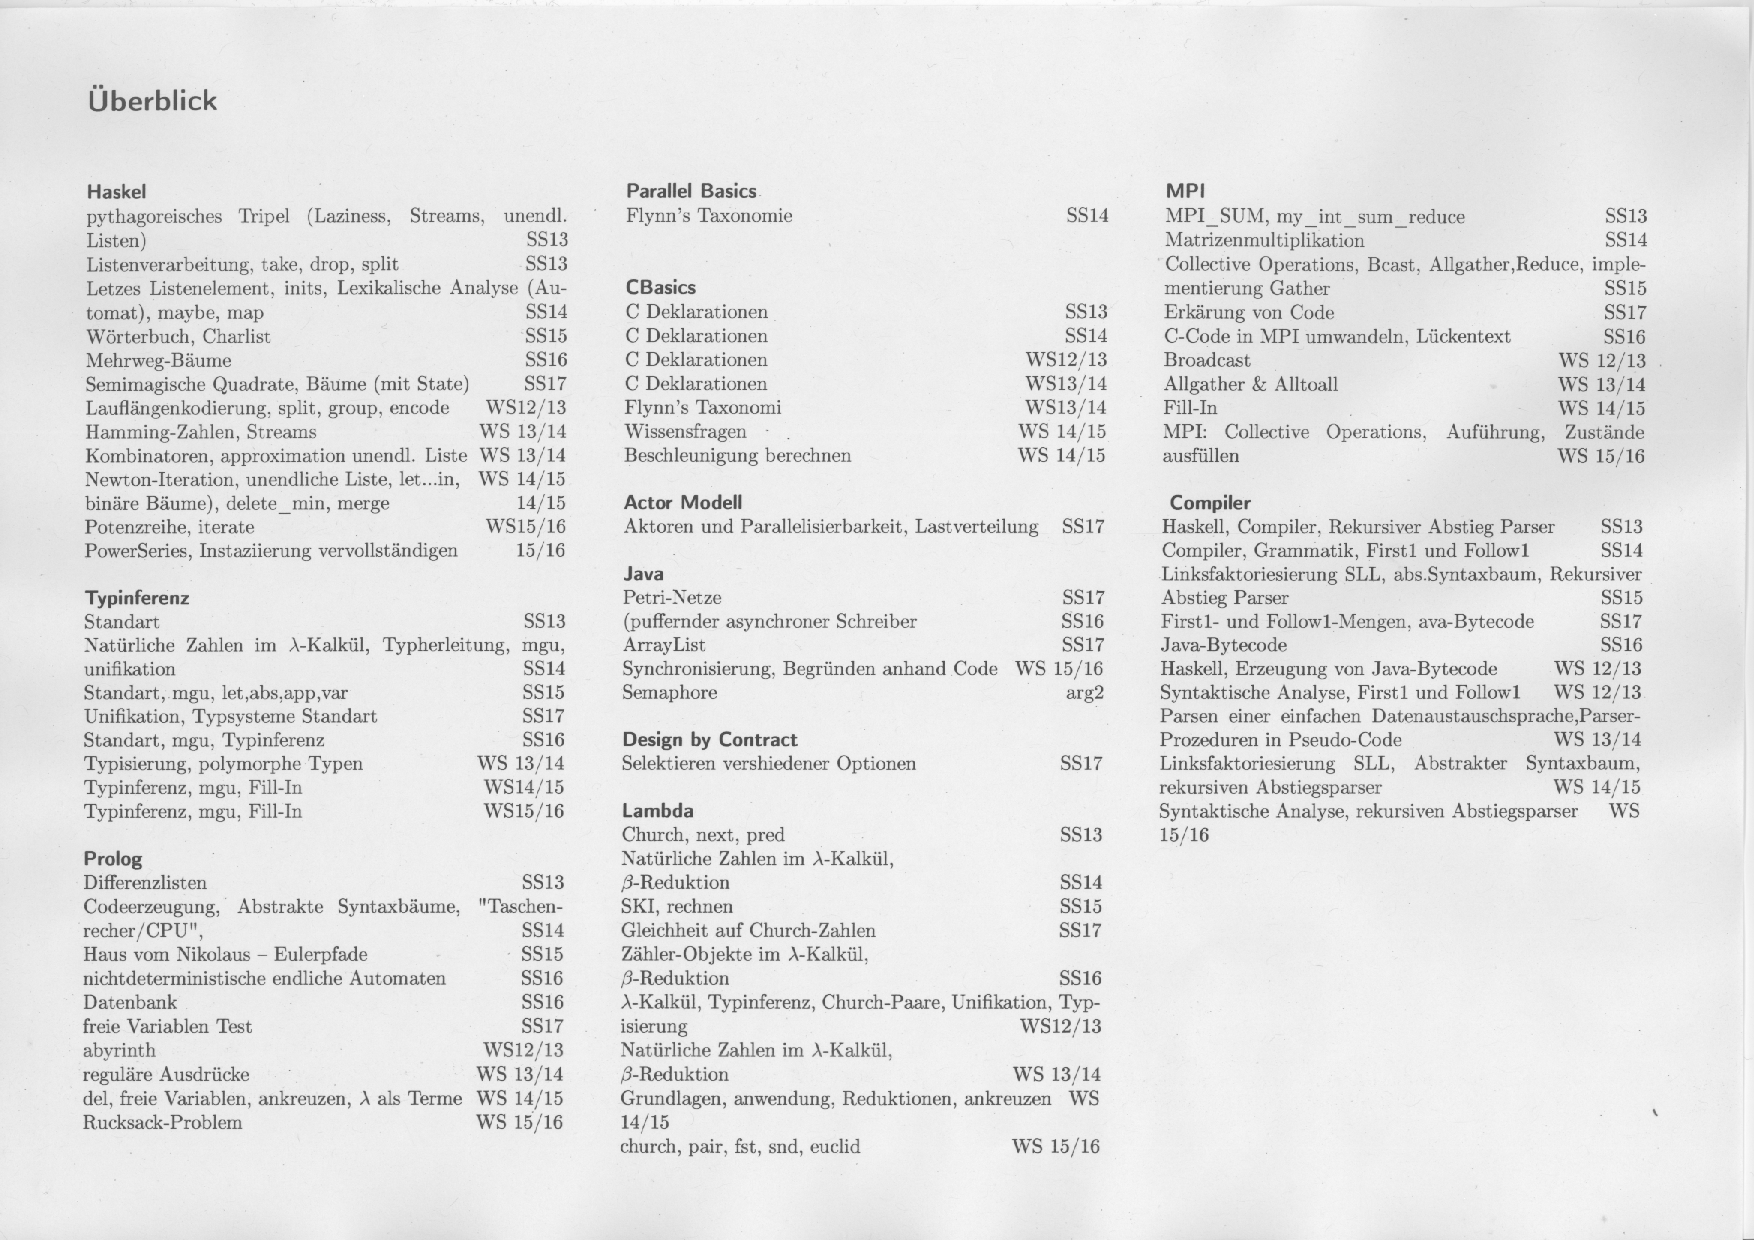
\includegraphics{imgs/TaskOverview.png}}
%\end{sidewaysfigure}

\subsection*{Haskell}
\begin{table}[h]
	\centering
	\begin{tabular}{l|l}
		\multlineTable{Bäume, mapTree, reduceTree / foldTree, treeSum,\\ treeConcat, treeToList}
		& WS 11 / 12 (Nr. 1) \\ \hline
		
		Hirsch-Index, Bäume, allTrees, trees\_4\_13
		& SS 12 (Nr. 1) \\ \hline
		
		Lauflängenenkodierung, splitWhen, group, encode 
		& WS 12 / 13 (Nr. 1)\\ \hline
		
		Java-Bytecode Erzeugung 
		& WS 12 / 13 (Nr. 8)\\ \hline
		
		Laziness, Streams, pythagoreisches Tripel 
		& SS 13 (Nr. 1)\\ \hline
		
		splits, alle möglichen Teillisten 
		& SS 13 (Nr. 4)\\ \hline
		
		Hamming-Zahlen 
		& WS 13 / 14 (Nr. 1)\\ \hline
		
		\multlineTable{Kombinatoren, unendliche Liste,\\ Eulerverfahren, iterate, zipWith }
		& WS 13 / 14 (Nr. 2)\\ \hline
		
		last (Listen-Element), inits 
		& SS 14 (Nr. 1)\\ \hline
		
		lexikalische Analyse, Maybe, Automat, Zahlensystem 
		& SS 14 (Nr. 2)\\ \hline
		
		Newton-Iteration
		& WS 14 / 15 (Nr. 1) \\ \hline
		
		binäre Bäume, deleteMin, merge Trees
		& WS 14 / 15 (Nr. 2) \\ \hline
		
		splitWords (Word, NonWord), joinWords, capitalize
		& SS 15 (Nr. 1) \\ \hline
		
		\multlineTable{Potenzreihe, iterate, addieren, multiplizieren,\\ differenzieren, evaluieren}
		& WS 15 / 16 (Nr. 1) \\ \hline
		
		Datentyp, Typ-Instanziierung
		& WS 15 / 16 (Nr. 2) \\ \hline
		
		\multlineTable{Mehrwegbäume, treeIndex, treePositions,\\ changeTree , overrideTree, i-tes Listen-Element}
		& SS 16 (Nr. 1) \\ \hline
		
		\multlineTable{semimagische Quadrate, Duplikate-Test, transponieren,\\ Überprüfung auf semimagisches Quadrat}
		& SS 17 (Nr. 1) \\ \hline
		
		Mehrweg-Bäume, tote \& lebendige Blätter, prune
		& SS 17 (Nr. 2) \\ \hline
	\end{tabular}
\end{table}
\FloatBarrier

\subsection*{Prolog}
\begin{table}[h]
	\centering
	\begin{tabular}{l|l}
		Nichtdeterminismus, Wechselgeld, removeMoney, changeMoney
		& WS 11 / 12  (Nr. 2)\\ \hline
				
		Wolf, Ziege, Kohl
		& SS 12 (Nr. 2)\\ \hline
		
		Labyrinth
		& WS 12 / 13 (Nr. 3)\\ \hline
		
		splits, alle möglichen Teillisten
		& SS 13 (Nr. 4)\\ \hline
		
		Differenzlisten
		& SS 13 (Nr. 5)\\ \hline
		
		reguläre Ausdrücke
		& WS 13 / 14 (Nr. 5) \\ \hline
		
		Java-Bytecodeerzeugung
		& SS 14 (Nr. 5) \\ \hline
		
		del, delete, freie Variablen in Lambda-Ausdruck
		& WS 14 / 15 (Nr. 4) \\ \hline
		
		Haus vom Nikolaus, Eulerpfade, swap (Kanten umdrehen)
		& SS 15 (Nr. 4) \\ \hline
		
		Rucksack-Problem, alle möglichen Teil-Listen
		& WS 15 / 16 (Nr. 3) \\ \hline
		
		nichtdeterministische endliche Automaten
		& SS 16 (Nr. 2) \\ \hline
		
		\multlineTable{Noten-Datenbank, Campus-Verwaltungssystem,\\ transitive Voraussetzung}
		& SS 16 (Nr. 3) \\ \hline
		
		freie Variablen
		& SS 17 (Nr. 3) \\ \hline
	\end{tabular}
\end{table}
\FloatBarrier
\newpage

\subsection*{$\lambda$-Kalkül}
\begin{table}[h]
\centering
\begin{tabular}{l|l}
	Fixpunktkombinator, $\beta$-Reduktion
	& WS 11 / 12  (Nr. 3)\\ \hline
	
	Kombinatoren, $\beta$-Reduktion, S K I
	& SS 12 (Nr. 3)\\ \hline
	
	Church-Paare, fst, snd, map, allgemeinster Typ
	& WS 12 / 13 (Nr. 2) \\ \hline
	
	Church-Paare, next, pred 
	& SS 13 (Nr. 2) \\ \hline
	
	Church-Zahlen, isZero, pred, add 
	& WS 13 / 14 (Nr. 3)\\ \hline
	
	Scott-Zahlen, isZero, pred, sub 
	& SS 14 (Nr. 3)\\ \hline
	
	\multlineTable{freie Variablen, Redex, call-by-name, Normalform,\\ $\alpha$- \& $\eta$-Äquivalenz }
	& WS 14 / 15 (Nr. 3) \\ \hline
	
	S K I, Normalform
	& SS 15 (Nr. 2) \\ \hline
	
	\multlineTable{Pair, fst, snd, swap (fst \& snd v. pair), Normalform,\\ euklidischer Algo, größter gemeinsamer Teiler,\\ Church-Zahlen}
	& WS 15 / 16 (Nr. 4) \\ \hline
	
	Church-Zahlen, inc, add, get, react
	& SS 16 (Nr. 4) \\ \hline
	
	Church-Zahlen, $c_{true}$, $c_{false}$, pred, Gleichheits-Test 
	& SS 17 (Nr. 6) \\ \hline
\end{tabular}
\end{table}
\FloatBarrier

\subsection*{Typinferenz}
\begin{table}[h]
\centering
\begin{tabular}{l|l}
	S K I, Let-Polymorphismus
	& WS 11 / 12  (Nr. 4) \\ \hline
	
	Unifikation, Prolog-Notation
	& SS 12 (Nr. 4) \\ \hline
	
	allgemeinster Typ, Typschema, let-Polymorphismus 
	& SS 13 (Nr. 3)\\ \hline
	
	let-Polymorphismus, $\lambda$-gebunde Variable $\rightarrow$ nicht polymorph 
	& WS 13 / 14 (Nr. 4)\\ \hline
	
	Scott-Zahlen, allgemeinster Typ, mgu 
	& SS 14 (Nr. 4)\\ \hline
	
	mgu, $\tau_{just}$, let-Polymorphismus
	& WS 14 / 15 (Nr. 5) \\ \hline
	
	mgu, let-Polymorphismus, $\lambda$-gebunde Variable $\rightarrow$ nicht polymorph
	& SS 15 (Nr. 3) \\ \hline
	
	mgu, allgemeinster Typ, Typabstraktion, let-Polymorphismus
	& WS 15 / 16 (Nr. 5) \\ \hline
	
	$C_0$ \& $C_{let}$, let-Polymorphismus, mgu
	& SS 16 (Nr. 5) \\ \hline
	
	Unifikation, ausgeschrieben
	& SS 17 (Nr. 4) \\ \hline
	
	$\lambda$-Term zu Typ erstellen, let-Polymorphismus, allgemeinster Typ
	& SS 17 (Nr. 5) \\ \hline
\end{tabular}
\end{table}
\FloatBarrier

\subsection*{Parallel Basics}
\begin{table}[h]
	\centering
	\begin{tabular}{l|l}		
		Flynn’s Taxonomie 
		& \multlineTable{WS 13 / 14 (Nr. 9)\\ SS 14 (Nr. 6)}\\ \hline		
		
		\multlineTable{Vorteile, Risiken, Thread-Scheduling, Sperren,\\ Race-Bedingung, Deadlock,\\ blocking vs. non-blocking, synchron-Send}
		& WS 14 / 15 (Nr. 6) \\ \hline			
		
		Beschleunigung berechnen, Amdahls Law
		& WS 14 / 15 (Nr. 7) \\ \hline		
				
		\multlineTable{Synchronisierung, Bank, Race-Condition,\\ Deadlock, synchronized, Coffman-Bedingungen}
		& WS 15 / 16 (Nr. 7) \\ \hline
	\end{tabular}
\end{table}
\FloatBarrier
\newpage

\subsection*{C}
\begin{compactitem}
	\item Zeiger-Arithmetik, Arrays \qquad WS 11 / 12 (Nr. 5),  SS 12 (Nr. 5)
	\item Precedence-Rule \qquad \qquad \qquad WS 12 / 13 (Nr. 4), SS 13 (Nr. 6), WS 13 / 14 (Nr. 6), SS 14 (Nr. 9)
\end{compactitem}

\subsection*{MPI}
\begin{table}[h]
	\centering
	\begin{tabular}{l|l}
		Array-Durchschnitt
		& WS 11 / 12  (Nr. 6)\\ \hline
		
		Matrix-Multiplikation
		& SS 12 (Nr. 6), SS 14 (Nr. 8) \\ \hline
		
		Broadcast-Implementierung
		& WS 12 / 13 (Nr. 6) \\ \hline
		
		Reduce, Reduce-Implementierung 
		& SS 13 (Nr. 7)\\ \hline
		
		Allgather \& Alltoall 
		& WS 13 / 14 (Nr. 7) \\ \hline	
		
		Scatterv / Gatherv
		& SS 14 (Nr. 8) \\ \hline		
		
		\multlineTable{Send, Recv, Finalize,\\ Parameter-Beschreibungen}
		& WS 14 / 15 (Nr. 9) \\ \hline	
		
		Gather-Implementierung
		& SS 15 (Nr. 5) \\ \hline
		
		Scatter, Allgather
		& WS 15 / 16 (Nr. 6) \\ \hline
		
		Scatter, Reduce, Lückentext
		& SS 16 (Nr. 8) \\ \hline
		
		Bcast, Reduce
		& SS 17 (Nr. 7) \\ \hline
	\end{tabular}
\end{table}
\FloatBarrier

\subsection*{Java}
\begin{table}[h]
	\centering
	\begin{tabular}{l|l}		
		\multlineTable{Synchronisierung, Bank, Race-Condition, Deadlock,\\ synchronized, Coffman-Bedingungen}
		& WS 15 / 16 (Nr. 7) \\ \hline
		
		Zähl-Semaphore, Monitore, Signalisierungsmethoden 
		& WS 15 / 16 (Nr. 8) \\ \hline
		
		\multlineTable{puffernder asynchroner Schreiber,\\ flushBuffer, isInterrupted}
		& SS 16 (Nr. 6) \\ \hline
		
		\multlineTable{ArrayList, synchronized,\\ Deadlock, Race-Condition}
		& SS 16 (Nr. 7) \\ \hline
		
		Worker-Balancer, Amdahls Law
		& SS 17 (Nr. 8) \\ \hline
		
		Petri-Netze, Token, Place, Deadlock, Coffman-Bedingungen
		& SS 17 (Nr. 9) \\ \hline
	\end{tabular}
\end{table}
\FloatBarrier

\subsection*{Design by Contract}
Optionen selektieren, deselektieren, if-else: SS 17 (Nr. 10) 

\subsection*{Compiler}
\begin{table}[h]
	\centering
	\begin{tabular}{l|l}
		\multlineTable{Syntaktische Analyse, abstrakte Syntax,\\ rekursiver Abstiegsparser}
		& \multlineTable{WS 11 / 12 (Nr. 8)\\ SS 12 (Nr. 6)} \\ \hline	
		
		Haskell, Java-Bytecode Erzeugung
		& WS 12 / 13 (Nr. 8) \\ \hline
		
		First-\& Follow-Mengen 
		& \multlineTable{WS 12 / 13 (Nr. 9)\\ SS 14 (Nr. 10)\\ SS 17 (Nr. 11)} \\ \hline	
		
		\multlineTable{Linksfaktorisierung, Haskell-Datentyp,\\ Abstiegsparser }
		& SS 13 (Nr. 9) \\ \hline
		
		Abstiegsparser 
		& WS 13 / 14 (Nr. 10) \\ \hline	
		
		\multlineTable{Linksfaktorisierung, SLL(1), abstrakte Syntax,\\ Klassenherarchie, Abstiegsparser}
		& WS 14 / 15 (Nr. 10) \\ \hline	
		
		\multlineTable{Linksfaktorisierung, abstrakte Syntax,\\ Abstiegsparser, abstrakter Syntaxbaum}
		& SS 15 (Nr. 2) \\ \hline
		
		Abstiegsparser 
		& WS 15 / 16 (Nr. 10) \\ \hline
		
		Java-Bytecode, if
		& SS 16 (Nr. 9) \\ \hline
	\end{tabular}
\end{table}
\FloatBarrier

\end{document}